\documentclass{beamer}
\usetheme{Berlin}
\usecolortheme{beaver}
\setbeamertemplate{itemize items}[square]
\setbeamercovered{transparent}
\setbeamertemplate{footline}[frame number]
\usepackage[ngerman]{babel}
\usepackage{graphicx}
\usepackage[utf8]{inputenc}
\usepackage{times}
\usepackage[T1]{fontenc}

\title[Session Talk]{Malware}
\author{}
\date{}

\begin{document}

\maketitle


\begin{frame}
\frametitle{Inhalt}

\begin{block}{Themen:}
\begin{enumerate}
\item Malware Statistik
\item Erkennungsrate vs. Infektionswahrscheinlichkeit
\item Performance-Efficiency-Tradeoff
\item Malware Scanning
\begin{itemize}
\item Static Scanning
\item Dynamic Scanning
\item Heuristic/Proactive Scanning
\end{itemize}
\end{enumerate}
\end{block}
\end{frame}

\section{Malware Statistik}
\begin{frame}
\frametitle{Statistik}

Neue Malware \\
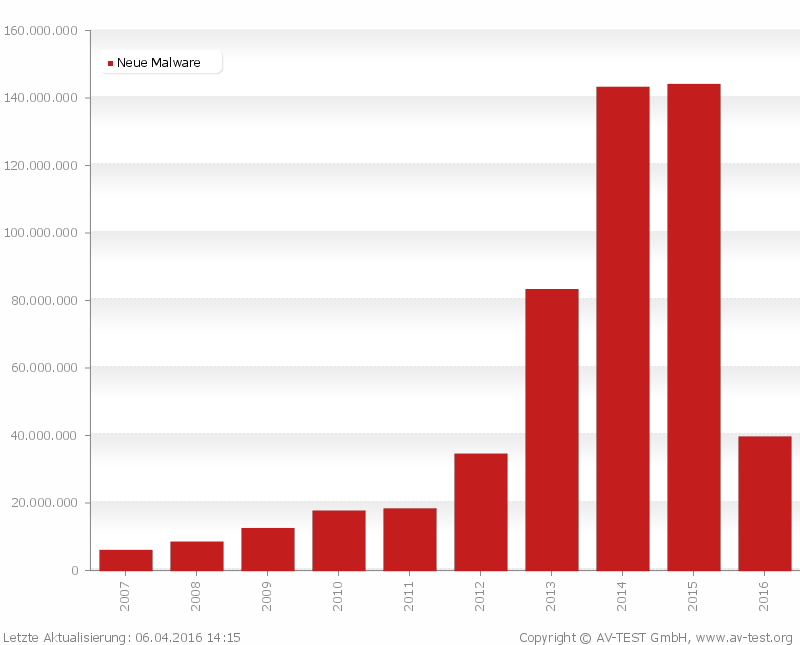
\includegraphics[height=7cm]{bilder/growth.png}
\end{frame}

\begin{frame}
\frametitle{Statistik}
Gesamte Malware \\
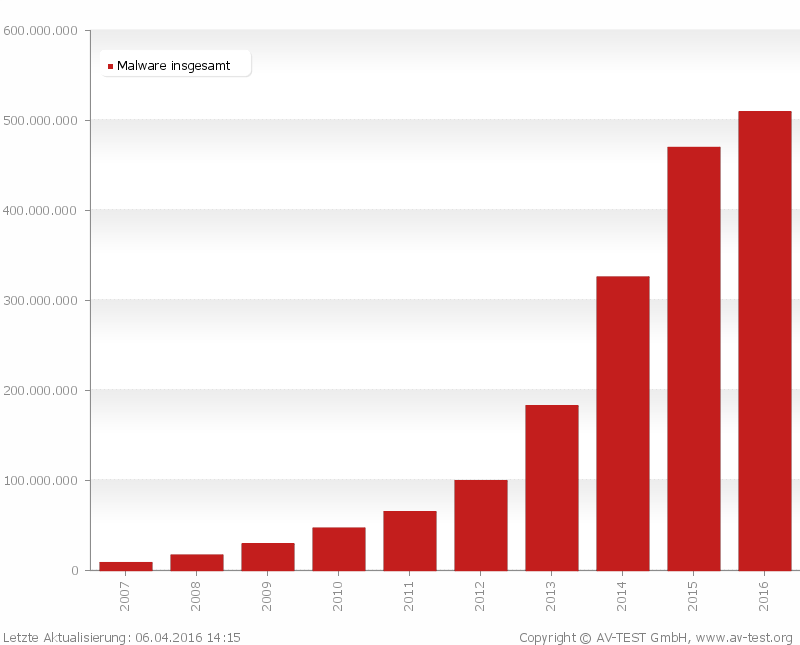
\includegraphics[height=7cm]{bilder/total.png}

\end{frame}

\begin{frame}
\frametitle{Statistik}
Ransomware \\
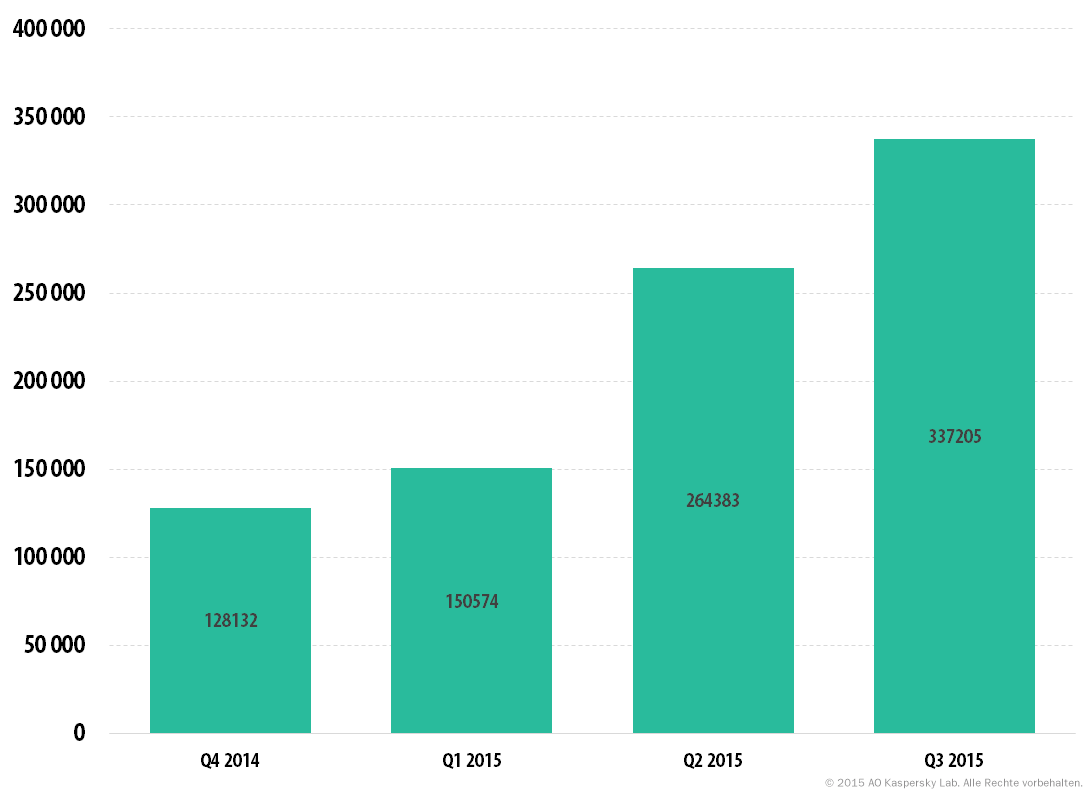
\includegraphics[height=7cm]{bilder/ransom.png}

\end{frame}



\section{Malware Scanning}
\begin{frame}
Hauptkriterien:
\begin{itemize}
	\item Erkennungsrate vs. Infektionswahrscheinlichkeit
	\item Performance-Effectivity-Tradeoff
	\item Scanning Techniken
\end{itemize}
\end{frame}

\begin{frame}
\frametitle{Erkennungsrate vs. Infektionswahrscheinlichkeit}
\begin{block}{}
	Infektionswahrscheinlichkeit != 1 - Erkennungsrate
\end{block}
Infektionswahrschinlichkeit bei $n$ voneinander unabh�ngige Angriffe: \\
\centering
$p_{Befall} = (r_x)^n$




\end{frame}

\begin{frame}
\frametitle{Performance-Effectivity-Tradeoff}
Hohe Effektivit�t -> hoher Leistungsverbrauch -> niedrige Performance \\
Hohe Performance -> niedriger Leistungsverbrauch -> niedrige Effektivit�t

Kompromiss zwischen Performance und Effektivit�t
	
\end{frame}

\section{Malware Scanning}

\begin{frame}
\frametitle{Malware Scanning}
\begin{block}{Static Scanning}
	\begin{enumerate}
		\item Codeausschnitt aus Datei
		\item Vergleich mit Codeausschnitten in Datenbank
		\item Entscheidung, ob Virus oder nicht
	\end{enumerate}

\end{block} 

\end{frame}
\begin{frame}
	\frametitle{Malware Scanning}
	\begin{block}{Vorteile}
		\begin{itemize}
			\item Erkennt Malware mit festgelegter Signatur garantiert
			\item Datei muss nicht ge�ffnet/ausgef�hrt werden
		\end{itemize}
	\end{block} 
	\begin{block}{Nachteile}
		\begin{itemize}
			\item �bersieht unbekannte Sch�dlinge
			\item Erkennt keine alternativen Versionen
			\item Erkennt nur exakte Treffer
			\item Speicherverbrauch f�r Datenbank
		\end{itemize}
	\end{block}
	
\end{frame}

\begin{frame}
\frametitle{Malware Scanning}
\begin{block}{Dynamic Scanning}
	\begin{enumerate}
		\item Verhalten in Verhaltenskatalog gespeichert
		\item �berpr�ft Verhalten bei �ffnen/Ausf�hren
		\item Vergleicht Verhalten mit Katalog
		\item Blockiert Programm oder l�sst Ausf�hrung zu
	\end{enumerate}
	
\end{block} 
\end{frame}

\begin{frame}
	\frametitle{Malware Scanning}
	\begin{block}{Vorteile}
		\begin{itemize}
			\item Unbekannte Malware kann erkannt werden
		\end{itemize}
	\end{block} 
	\begin{block}{Nachteile}
		\begin{itemize}
			\item Schwierig alle Verhaltensweisen festzuhalten
			\item Kann evtl. Verhalten nicht erkennen
			\item Kann keine v�llig neuen Sch�dlinge erkennen
			\item False-Positives: Blockiert gutartige Programme
		\end{itemize}
	\end{block}
	
\end{frame}


\begin{frame}
\frametitle{Malware Scanning}
\begin{block}{Heuristic/Proaktive Scanning}
	\begin{itemize}
		\item Bestimmt Wahrscheinlichkeit sch�dlichen Verhaltens
		\item F�hrt Datei nicht aus
		\item blockiert Programm aufgrund berechneter Wahrscheinlichkeit
	\end{itemize}
		
\end{block} 

\end{frame}




\begin{frame}
	\frametitle{Scanner umgehen}
	Malware kann nur gefunden werden wenn:
	\begin{itemize}
		\item Signatur in der Datenbank existiert
		\item Verhalten in der Datenbank existiert
		\item Heuristische Untersuchung eine hohe Wahrscheinlichkeit f�r sch�dliches Verhalten ermitteln
	\end{itemize}
	Design neuer Malware:
	\begin{itemize}
		\item Neue Signatur oder komplett neues Verhalten kann von keinem Scanner erkannt werden.
		\item Gefahr besteht, bis �nderungen in Anti-Malware integriert.
		\item Integration von Signaturen schnell, von Verhaltensregeln langsam.
		\item Bis zur Aktualisierung: kein Schutz
	\end{itemize}
	
	
	
	
\end{frame}



\begin{frame}
	\frametitle{Schlussfolgerung}
	Gute Scanner muss:
	\begin{itemize}
		\item alle Scanning-Techniken Kombinieren
		\item dadurch eine sehr hohe Erkennungsrate haben
		\item einen Kompromiss zwischen Performance und Effizienz finden
		\item Regelm��ig mit Updates versorgt werden.
	\end{itemize}
	\begin{block}{}
		Trotz der Erf�llung dieser Voraussetzungen sitzen Malware Entwickler immer am l�ngeren Ast. Wird eine Komplett neuartige Malware entwickelt, muss diese erst identifiziert, sowie Regeln und Signaturen daf�r erstellt werden. Bis zu dem Zeitpunkt, zu dem das Update an User ausgeliefert wird, sind deren Ger�te der neuen Malware Schutzlos ausgeliefert
		
	\end{block}



\end{frame}



\end{document}
